%%%%%%%%%%%%%%%%%%%%%%%%%%%%%%%%
\section{Experimental evaluation}
\label{fi:sec:experimental}

In this section, we compare \LSR{} and \ILSR{} to other inference algorithms in terms of
\begin{enuminline}
\item statistical efficiency, and
\item empirical performance.
\end{enuminline}
In order to understand the efficiency of the estimators, we generate synthetic data from a known ground truth.
Then, we look at five real-world datasets and investigate the practical performance of the algorithms in terms of accuracy, running time and convergence rate.

\paragraph{Error metric.}
As the probability of $i$ winning over $j$ depends on the ratio of strengths $\pi_i / \pi_i$, the strengths are typically logarithmically spaced.
In order to evaluate the accuracy of an estimate $\bm{\pi}$ to ground truth parameters $\bm{\pi}^*$, we therefore use a $\log$ transformation, reminiscent of the random-utility-theoretic formulation of the choice model \citep{mcfadden1973conditional,hajek2014minimax}.
Define $\bm{\theta} \doteq[\log \pi_i - t]$, with $t$ chosen such that $\sum_i \theta_i = 0$.
We will consider the root-mean-squared error (RMSE)
\begin{align*}
E_{\text{RMS}} = \Vert \bm{\theta} - \bm{\theta}^* \Vert_2 / \sqrt{n}.
\end{align*}

\subsection{Statistical efficiency}

To assess the statistical efficiency of \LSR{} and other algorithms, we follow the experimental procedure of \citet{hajek2014minimax}.
We consider $n = 1024$ items, and draw $\bm{\theta}^*$ uniformly at random in $[-2, 2]^n$.
We generate $d = 64$ full rankings over the $n$ items from a Plackett-Luce model parametrized with $\bm{\pi} \propto [e^{\theta_i}]$.
For a given $k \in \{2^1, \ldots, 2^{10}\}$, we break down each of the full rankings as follows.
First, we partition the items into $n/k$ subsets of size $k$ uniformly at random.
Then, we store the $k$-way rankings induced by the full ranking on each of those subsets.
As a result, we obtain $m = dn/k$ statistically independent $k$-way partial rankings.
For a given estimator, this data produces an estimate $\bm{\theta}$, for which we record the root-mean-square error to $\bm{\theta}^*$.
We consider four estimators.
The first two (\LSR{} and ML) work on the ranking data directly.
The remaining two follow \citet{azari2013generalized}, who suggest breaking down $k$-way rankings into $\binom{k}{2}$ pairwise comparisons.
These comparisons are then used by \LSR{}, resulting in \citeauthor{azari2013generalized}'s GMM-F estimator, and by an ML estimator (ML-F.)
In short, the four estimators vary according to
\begin{enuminline}
\item whether they use as-is rankings or derived comparisons, and
\item whether the model is fitted using an approximate spectral algorithm or using exact maximum likelihood.
\end{enuminline}
Figure~\ref{fi:fig:efficiency} plots $E_{\text{RMS}}$ for increasing sizes of partial rankings, as well as a lower bound to the error of any estimator for the Plackett-Luce model (see \citet{hajek2014minimax} for details.)
We observe that breaking the rankings into pairwise comparisons (*-F estimators) incurs a significant efficiency loss over using the $k$-way rankings directly (\LSR{} and ML.)
We conclude that by correctly weighting pairwise rates in the Markov chain, \LSR{} distinctly outperforms the rank-breaking approach as $k$ increases.
We also observe that the ML estimate is always more efficient.
Spectral estimators such as \LSR{} provide a quick, asymptotically consistent estimate of parameters, but this observation justifies calling them \emph{approximate} inference algorithms.


\begin{figure}[ht]
%\vskip -0.1in
\centering
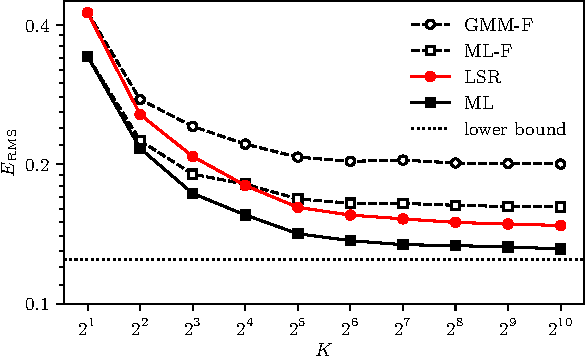
\includegraphics{fi-efficiency}
\vskip -0.1in
\caption{
Statistical efficiency of different estimators for increasing sizes of partial rankings.
As $k$ grows, breaking rankings into pairwise comparisons becomes increasingly inefficient.
\LSR{} remains efficient at no additional computational cost.
}
\vskip -0.1in
\label{fi:fig:efficiency}
\end{figure}

\subsection{Empirical performance}

We investigate the performance of various inference algorithms on five real-world datasets.
The NASCAR \citep{hunter2004mm} and sushi \citep{kamishima2009efficient} datasets contain multiway partial rankings.
The YouTube, GIFGIF and chess datasets\footnote{
See \url{https://archive.ics.uci.edu/ml/machine-learning-databases/00223/}, \url{http://www.gif.gf/} and \url{https://www.kaggle.com/c/chess}.
} contain pairwise comparisons.
Among those, the chess dataset is particular in that it features 45\% of ties;
in this case we use the extension of the Bradley--Terry model proposed by \citet{rao1967ties}.
We preprocess each dataset by discarding items that are not part of the largest strongly connected component in the comparison graph.
The number of items $n$, the number of rankings $m$, as well as the size of a partial rankings $k$ for each dataset are given in Table~\ref{fi:tab:approxalg}.
Additional details on the experimental setup are given in the supplementary material.
We first compare the estimates produced by three approximate ML inference algorithms, \LSR{}, GMM-F and Rank Centrality (RC.)
Note that RC applies only to pairwise comparisons, and that \LSR{} is the only algorithm able to infer the parameters in the Rao-Kupper model.
Also note that in the case of pairwise comparisons, GMM-F and \LSR{} are strictly equivalent.
In Table~\ref{fi:tab:approxalg}, we report the root-mean-square deviation to the ML estimate $\hat{\bm{\theta}}$ and the running time $T$ of the algorithm.

\sisetup{group-minimum-digits=4,detect-weight=true}
\begin{table}[ht]
  \vspace{-0.3cm}
  \caption{Performance of approximate ML inference algorithms}
  \label{fi:tab:approxalg}
  \centering
  \small{
  \begin{tabular}{l rrr rr rr rr rr}
    \toprule
            &             &               &          & \multicolumn{2}{c}{\LSR{}}            & \multicolumn{2}{c}{GMM-F}          & \multicolumn{2}{c}{RC} \\
                                                       \cmidrule(l){5-6}                    \cmidrule(l){7-8}                    \cmidrule(l){9-10}
    Dataset &         $n$ &           $m$ &      $k$ &     $E_{\text{RMS}}$ &     $T$ [s] &     $E_{\text{RMS}}$ &     $T$ [s] & $E_{\text{RMS}}$ & $T$ [s] \\
    \midrule
    NASCAR  &    \num{83} &      \num{36} & \num{43} & \bfseries\num{0.194} &  \num{0.03} &          \num{0.751} &  \num{0.06} &         --- &         --- \\
    Sushi   &   \num{100} &    \num{5000} & \num{10} & \bfseries\num{0.034} &  \num{0.22} &          \num{0.130} &  \num{0.19} &         --- &         --- \\
    \addlinespace                                                                                                             
    YouTube & \num{16187} & \num{1128704} &  \num{2} & \bfseries\num{0.417} & \num{34.18} & \bfseries\num{0.417} & \num{34.18} & \num{0.432} & \num{41.91} \\
    GIFGIF  &  \num{5503} &   \num{95281} &  \num{2} & \bfseries\num{1.286} &  \num{1.90} & \bfseries\num{1.286} &  \num{1.90} & \num{1.295} &  \num{2.84} \\
    \addlinespace                                                                                                             
    Chess   &  \num{6174} &   \num{63421} &  \num{2} & \bfseries\num{0.420} &  \num{2.90} &                  --- &         --- &         --- &         --- \\
    \bottomrule
  \end{tabular}
  }
\end{table}

The smallest value of $E_{\text{RMS}}$ is highlighted in bold for each dataset.
We observe that in the case of multiway partial rankings, \LSR{} is almost four times more accurate than GMM-F on the datasets considered.
In the case of pairwise comparisons, RC is slightly worse than \LSR{} and GMM-F, because the number of comparisons per pair is not homogeneous (see Section~\ref{fi:sec:pairwise}.)
The running time of the three algorithms is comparable.

Next, we turn our attention to ML inference and consider three iterative algorithms: \ILSR{}, MM and Newton-Raphson.
For Newton-Raphson, we use an off-the-shelf solver.
Each algorithm is initialized with $\bm{\pi}^{(0)} = [1/n, \ldots, 1/n]^\intercal$, and convergence is declared when $E_{\text{RMS}} < 0.01$.
In Table~\ref{fi:tab:mlalg}, we report the number of iterations $I$ needed to reach convergence, as well as the total running time $T$ of the algorithm.

\begin{table}[ht]
  \vspace{-0.3cm}
  \caption{Performance of iterative ML inference algorithms.}
  %The algorithms are stopped when the estimate has a RMSE $< 0.01$.}
  \label{fi:tab:mlalg}
  \centering
  \small{
  \begin{tabular}{l r rr rr rr}
    \toprule
             &             & \multicolumn{2}{c}{\ILSR{}}        & \multicolumn{2}{c}{MM}      & \multicolumn{2}{c}{Newton} \\
                             \cmidrule(l){3-4}                  \cmidrule(l){5-6}             \cmidrule(l){7-8}
    Dataset  & $\gamma_{\mathcal{D}}$ & $I$ &         $T$ [s] &        $I$ &        $T$ [s] &     $I$ &     $T$ [s] \\
    \midrule
    NASCAR   & \num{0.832} &  \num{3} &   \bfseries\num{0.08} &    \num{4} &     \num{0.10} &     --- &         --- \\
    Sushi    & \num{0.890} &  \num{2} &   \bfseries\num{0.42} &    \num{4} &     \num{1.09} & \num{3} & \num{10.45} \\
    \addlinespace
    YouTube  & \num{0.002} & \num{12} & \bfseries\num{414.44} & \num{8680} & \num{22443.88} &     --- &         --- \\
    GIFGIF   & \num{0.408} & \num{10} &  \bfseries\num{22.31} &  \num{119} &   \num{109.62} & \num{5} & \num{72.38} \\
    \addlinespace
    Chess    & \num{0.007} & \num{15} &  \bfseries\num{43.69} &  \num{181} &    \num{55.61} & \num{3} & \num{49.37} \\
    \bottomrule
  \end{tabular}
  }
\end{table}

The smallest total running time $T$ is highlighted in bold for each dataset.
We observe that Newton-Raphson does not always converge, despite the log-likelihood being strictly concave\footnote{
On the NASCAR dataset, this has also been noted by \citet{hunter2004mm}.
Computing the Newton step appears to be severely ill-conditioned for many real-world datasets.
We believe that it can be addressed by a careful choice of starting point, step size, or by monitoring the numerical stability;
however, these modifications are non-trivial and impose an additional burden on the practitioner.
}.
\ILSR{} consistently outperforms MM and Newton-Raphson in running time.
Even if the average running time per iteration is in general larger than that of MM, it needs considerably fewer iterations:
For the YouTube dataset, \ILSR{} yields an increase in speed of over $50$ times.

The slow convergence of minorization-maximization algorithms is known \cite{hunter2004mm}, yet the scale of the issue and its apparent unpredictability is surprising.
In Hunter's MM algorithm, updating a given $\pi_i$ involves only parameters of items to which $i$ has been compared.
Therefore, we speculate that the convergence rate of MM is dependent on the expansion properties of the comparison graph $G_{\mathcal{D}}$.
As an illustration, we consider the sushi dataset.
To quantify the expansion properties, we look at the spectral gap $\gamma_{\mathcal{D}}$ of a simple random walk on $G_{\mathcal{D}}$;
intuitively, the larger the spectral gap is, the better the expansion properties are \citep{levin2008markov}.
The original comparison graph is almost complete, and $\gamma_{\mathcal{D}} = 0.890$.
By breaking each $10$-way ranking into $5$ independent pairwise comparisons, we effectively sparsify the comparison graph.
As a result, the spectral gap decreases to $0.784$.
In Figure~\ref{fi:fig:convergence}, we show the convergence rate of MM and \ILSR{} for the original ($k = 10$) and modified ($k = 2$) datasets.
We observe that both algorithms display linear convergence, however the rate at which MM converges appears to be sensitive to the structure of the comparison graph.
In contrast, \ILSR{} is robust to changes in the structure.
The spectral gap of each dataset is listed in Table~\ref{fi:tab:mlalg}.
%Therefore, to better interpret the result of Table~\ref{fi:tab:mlalg}, we also list for each dataset the spectral gap of its comparison graph.


\begin{figure}[ht]
\centering
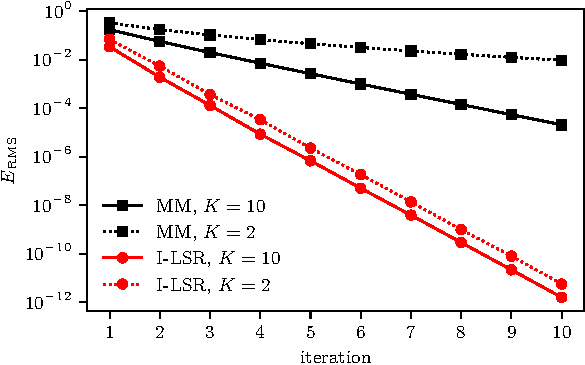
\includegraphics{fi-convergence}
\caption{
Convergence rate of \ILSR{} and MM on the sushi dataset.
When partial rankings ($k = 10$) are broken down into independent comparisons ($k = 2$), the comparison graph becomes sparser.
\ILSR{} is robust to this change, whereas the convergence rate of MM significantly decreases.
}
\label{fi:fig:convergence}
%\vskip -0.25in
\end{figure}
